% ============================================================
%  TERM PROJECT — USER MANUAL
%  Databases · THGA Bochum
% ============================================================
\documentclass[11pt,a4paper]{article}

\usepackage{thga-db}
\usepackage{graphicx}
\usepackage{float}

\renewcommand{\thgaKurs}{Databases}
\renewcommand{\thgaDatum}{Summer Term 2026}

\begin{document}
\thispagestyle{empty}

\thgaTitel{Term Project — User Manual}%
{VPN Access Manager: managing gateway sessions}

\begin{infobox}
\textbf{Author:} Rayen Ben Haj Rhouma \\
\textbf{Module:} Introduction to Database Management Systems · THGA Bochum \\
\textbf{Application:} VPN Access Manager, desktop client version 0.1.0 \\
\textbf{Repository:} \url{https://github.com/Rayen-CyberSecurity/vpn-access-manager}
\end{infobox}

\tableofcontents
\vspace{1em}

% ============================================================
\section{What this program does}
% ============================================================

VPN Access Manager is a desktop application for viewing and managing VPN
sessions.

It allows an administrator to:

\begin{itemize}
    \item see all configured VPN gateways,
    \item see how many active sessions each gateway currently has,
    \item view active and closed sessions,
    \item inspect the details of one session,
    \item open a new VPN session,
    \item close an active session.
\end{itemize}

Each gateway has a maximum number of simultaneous sessions. If that maximum is
reached, the application refuses additional sessions on that gateway.

The desktop application communicates only with the REST API. It does not
connect directly to the PostgreSQL database.

% ============================================================
\section{Installation}
% ============================================================

The client is distributed as a Debian package for 64-bit Linux.

Install it with:

\begin{verbatim}
sudo apt install ./vpn-manager_0.1.0_amd64.deb
\end{verbatim}

After installation, the application can be started from a terminal with:

\begin{verbatim}
vpn-manager
\end{verbatim}

It is also available as \textbf{VPN Access Manager} in the application menu.

To remove the client:

\begin{verbatim}
sudo apt remove vpn-manager
\end{verbatim}

To use the program, you need the URL of a running VPN Access Manager API and a
valid API key for operations that modify data.

% ============================================================
\section{Connecting to the server}
% ============================================================

When the application starts, it first displays the connection dialog.

\begin{figure}[H]
\centering
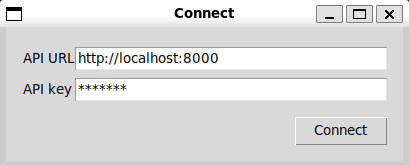
\includegraphics[width=0.6\textwidth]{img/fe-connect.png}
\caption{Connection dialog of the VPN Access Manager.}
\end{figure}

The dialog contains two fields:

\begin{description}
    \item[API URL]
    Address of the REST API, for example
    \texttt{http://localhost:8000}.

    \item[API key]
    Key used for operations that modify data. The value is hidden while it is
    entered and is kept only in memory while the program is running.
\end{description}

Click \textbf{Connect} to open the main application.

If the API cannot be reached, an error message is displayed.

\begin{figure}[H]
\centering
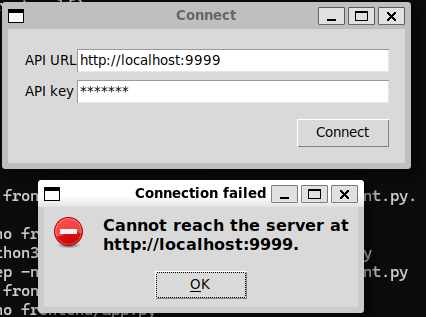
\includegraphics[width=0.6\textwidth]{img/fe-error-connection.png}
\caption{Error message when the API server cannot be reached.}
\end{figure}

Check the server address and verify that the API is running before trying
again.

% ============================================================
\section{Main window}
% ============================================================

After a successful connection, the main window is displayed.

\begin{figure}[H]
\centering
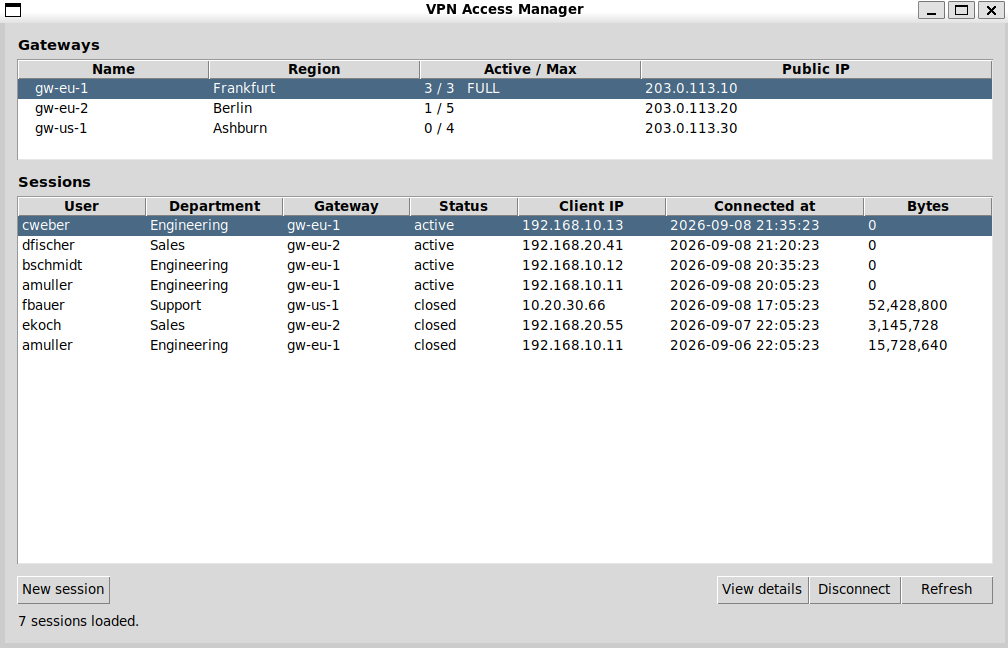
\includegraphics[width=\textwidth]{img/fe-main.png}
\caption{Main window showing gateways and VPN sessions.}
\end{figure}

The window contains two main tables.

\subsection*{Gateway overview}

The upper table displays:

\begin{itemize}
    \item gateway name,
    \item region,
    \item current number of active sessions,
    \item maximum allowed sessions,
    \item public IP address.
\end{itemize}

The \textbf{Active / Max} column shows the current load of each gateway.

For example,

\begin{verbatim}
3 / 3
\end{verbatim}

means that the gateway is full and cannot accept another session until an
active session is closed.

A gateway with zero active sessions is still displayed.

\subsection*{Session list}

The lower table displays stored VPN sessions, including both active and closed
sessions.

Each row shows information such as:

\begin{itemize}
    \item user,
    \item department,
    \item gateway,
    \item status,
    \item client IP,
    \item connection time,
    \item transferred bytes.
\end{itemize}

An \texttt{active} session is currently open.

A \texttt{closed} session remains in the database as historical information.

\subsection*{Available actions}

The buttons at the bottom of the window are:

\begin{description}
    \item[New session]
    Open a new VPN session.

    \item[View details]
    Display all available information for the selected session.

    \item[Disconnect]
    Close the selected active session.

    \item[Refresh]
    Reload gateway and session data from the REST API.
\end{description}

% ============================================================
\section{Opening a new session}
% ============================================================

Click \textbf{New session} in the main window.

The following dialog is displayed:

\begin{figure}[H]
\centering
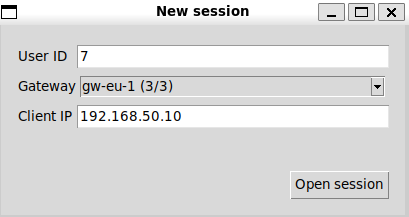
\includegraphics[width=0.6\textwidth]{img/fe-second.png}
\caption{Dialog for opening a new VPN session.}
\end{figure}

The fields are:

\begin{description}
    \item[User ID]
    Database identifier of the VPN user.

    \item[Gateway]
    Gateway on which the session should be opened. The current number of active
    sessions and maximum capacity are shown next to the gateway name.

    \item[Client IP]
    IPv4 address of the client opening the VPN connection, for example
    \texttt{192.168.50.10}.
\end{description}

After entering the values, click \textbf{Open session}.

If the input is valid and the selected gateway still has capacity, the session
is created and the main window is refreshed.

% ============================================================
\section{Gateway capacity error}
% ============================================================

A gateway cannot exceed its configured maximum number of active sessions.

If a gateway is already full, the API refuses the request and the frontend
displays the returned error message.

\begin{figure}[H]
\centering
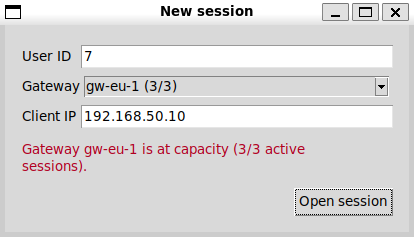
\includegraphics[width=0.7\textwidth]{img/fe-capacity-error.png}
\caption{Attempt to open a session on a gateway that has reached its capacity.}
\end{figure}

For example, a gateway showing

\begin{verbatim}
3 / 3
\end{verbatim}

already contains three active sessions and has a maximum capacity of three.

The user must either select another gateway or close an existing active session
before trying again.

% ============================================================
\section{Viewing session details}
% ============================================================

Select a session in the main table and click \textbf{View details}.

\begin{figure}[H]
\centering
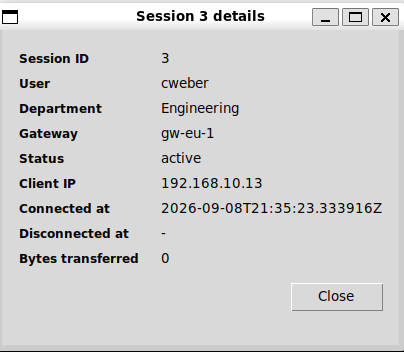
\includegraphics[width=0.65\textwidth]{img/fe-detail.png}
\caption{Detailed information for a selected VPN session.}
\end{figure}

The detail window shows:

\begin{itemize}
    \item session ID,
    \item user,
    \item department,
    \item gateway,
    \item session status,
    \item client IP,
    \item connection time,
    \item disconnection time,
    \item transferred bytes.
\end{itemize}

For an active session, the disconnection time is not yet available.

% ============================================================
\section{Closing a session}
% ============================================================

To close an active session:

\begin{enumerate}
    \item select the active session in the session table,
    \item click \textbf{Disconnect},
    \item confirm the operation.
\end{enumerate}

Before modifying the session, the program displays a confirmation dialog.

\begin{figure}[H]
\centering
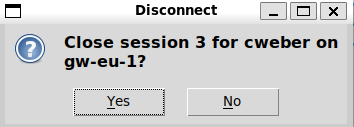
\includegraphics[width=0.6\textwidth]{img/fe-confirm-closed.png}
\caption{Confirmation before closing an active VPN session.}
\end{figure}

Click \textbf{Yes} to close the session.

The session is not deleted. Instead:

\begin{itemize}
    \item its status changes from \texttt{active} to \texttt{closed},
    \item its disconnection time is stored,
    \item its transferred byte value is stored,
    \item it remains visible in the session history.
\end{itemize}

The active-session count of the gateway decreases by one.

\begin{figure}[H]
\centering
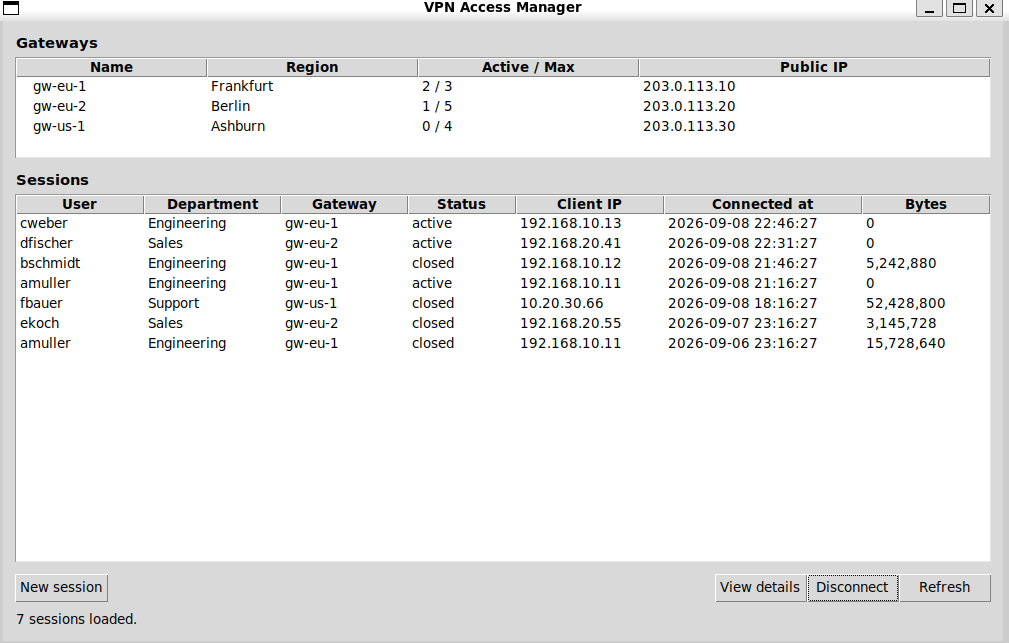
\includegraphics[width=\textwidth]{img/fe-after-close.png}
\caption{Main window after closing a session. The gateway has available capacity again.}
\end{figure}

Closing an already closed session does not modify its original closing
information.

% ============================================================
\section{Refreshing the data}
% ============================================================

The desktop client does not automatically poll the API.

If another administrator modifies the data, click \textbf{Refresh} to retrieve
the current gateway and session state.

This reloads both tables from the server.

% ============================================================
\section{Common problems}
% ============================================================

\begin{description}

\item[The server cannot be reached.]
Check that the API URL is correct and that the Docker services are running.

\item[I can view data but cannot open or close sessions.]
Read operations do not require an API key. Write operations require a valid
\texttt{X-API-Key}.

\item[The gateway is full.]
Select another gateway or close one of its active sessions.

\item[The client IP is rejected.]
Enter a valid IPv4 address such as \texttt{192.168.50.10}.

\item[The displayed data looks outdated.]
Click \textbf{Refresh} to reload the information from the server.

\item[Can a closed session be deleted from the desktop application?]
No. Closed sessions remain stored as historical records.

\end{description}

% ============================================================
\section*{Getting help}
% ============================================================

Problems can be reported at:

\url{https://github.com/Rayen-CyberSecurity/vpn-access-manager/issues}

Include the error message and the operation being performed, but never include
the API key.

\end{document}
